\documentclass[a4paper, 13pt]{article}
\usepackage[a4paper,top=50pt,bottom=50pt,left=30pt,right=30pt]{geometry}

\usepackage[french]{babel}

\usepackage{mathptmx}
\usepackage{enumitem}
\usepackage{graphicx}
\usepackage{hyperref}
\hypersetup{
    colorlinks=true,
    linkcolor=blue,
    urlcolor=blue,
}
\newcommand{\q}[1]{``#1''}
\begin{document}
\title{Compte rendu de la séance 3}
\author{Ecaterina GUPCA, Alice MERAUD, Jean COSTREL DE CORAINVILLE, Romain REN et Faustin MILLET}
\maketitle

\section{Compte rendu vidéo 3}
\subsection{La diffusion}
La diffusion est l’activité qui touche à la promotion et la commercialisation des livres.
\subsection{Le marché visé}
Le réseau des libraires est composé des libraires indépendants, chaînes, coopérations avec le milieu scolaire. Avec un grand nombre de livres, les diffuseurs propagent au maximum l'information pour faire vendre au maximum. Le diffuseur travaille aussi directement sur le terrain, on peut le voir notamment dans des grandes surfaces, magasins ayant un rayon dédié aux livres, boutiques spécialisées, marchands de journaux.
\subsection{L’office}
L'office est le mode d'approvisionnement des libraires.
Les libraires concernés reçoivent tous les nouveaux livres, journaux, etc qui les concernent (qu'ils ont demandés ou qui les intéresseraient). Le diffuseur met au point une grille d’office, avec le libraire qui indique le type, la quantité de livres qui serait envoyé aux librairies à partir du pontentiel profit de la librairie. Le représentant du diffuseur lui communique.
Les pré-notés sont des quantités de biens qui sont modifiés de la grille d’office sur un accord commun entre le libraire et le diffuseur lors des nouvelles apparitions. 
Les frais de livraisons sont prises en charges par le diffuseur et le client possède le droit de retour des livres non désiré.
Le système de la loi d’office permet de donner une certaine visibilité aux libraires. C’est une opportunité immanquable pour les libraires.  
\subsection{Commercialisation des fonds}
\begin{itemize}
    \item Mise en place des différents modes de commercialisations
    \item La promotion et la consignation (consignation aux libraires)  
    \item Lorsque le client commande des livres auprès des diffuseurs ou des distributeurs
    \item Le réassort (réapprovisionnement selon la forte demande)
\end{itemize}

\subsection{Les moyens d’actions}
Différents outils de diffusions : affiches, catalogues, des présentations publicitaires.
Les diffuseurs fournissent des infos statistiques aux libraires concernant les historiques d’un type de livres, titres, collections, etc. Certains diffuseurs disposent de bulletin d’informations ou utilise leurs sites internet enfin pour diffuser les informations, les diffuseurs invitent les libraires aux salons littéraires au début de saison pour qu'ils puissent s'informer sur les nouveautés et sorties de l’année.
\subsection{Le représentant}
Le représentant fait la passerelle directe entre le diffuseur et le détaillant, son travail consiste à présenter les nouveaux livres sortis sur le marché, mais aussi de consulter les libraires pour déterminer l'évolution de leurs ventes et voir comment faire évoluer ces chiffres, mettre en place divers moyens d’actions pour soutenir leur développement.
\subsection{Service de Presse}
Les médias ont un impact important sur le marché des livres. Certains diffuseurs ont la permission de prendre contact direct avec les médias pour représenter les libraires ou les éditeurs. Pour cela les représentants doivent avoir une connaissance fine et une culture littéraire riche.
\subsection{Les salons des livres}
Les diffuseurs réservent des espaces lors de la saison de la littérature pour promouvoir la production éditoriale. L’existence des salons du livre est propre au marché canadien/français et au Québec.
Il existe 9 salons en Québec.
\section{Compte rendu vidéo 4}

La distribution se définie comme la logistique de l'acheminement des livres vers le lieu de vente.
Pour un distributeur le centre de distribution est une partie essentielle, où se trouve toutes les opérations principales liées à la distribution, avec la réception des stocks, entreposage de la marchandise, gestion des commandes et des retours.
Dans un premier temps le stock des distributeurs provienne des éditeurs, ou bien directement par les imprimeurs. Les stocks transportés en quantité jusqu'au lieu d'entreposage, les transports peuvent être faits par bateau ou par avion dans les cas d'urgence, mais augmente des coûts.
Les livres sont vérifiés, emboîtés et séparés en deux catégories, les stocks légers pour répondre à des demandes à court terme et les stocks lourds pour des demandes à plus long terme.
Pour répondre aux commandes, les distributeurs s'occupent de les préparer, les met en boites, puis les commandes sont récupérées directement par les détaillants, mais souvent exportées via l'entreprise de transporteur de leurs choix. Le distributeur doit aussi gérer la gestion des retours.
Les distributeurs doivent gérer la base de données, les informations commerciales relatives à chaque document. Le distributeur doit la tenir à jour et l’exploiter. Cette base de données doit contenir par exemple le nombre d'exemplaires.
\begin{figure}[h]
    \centering
    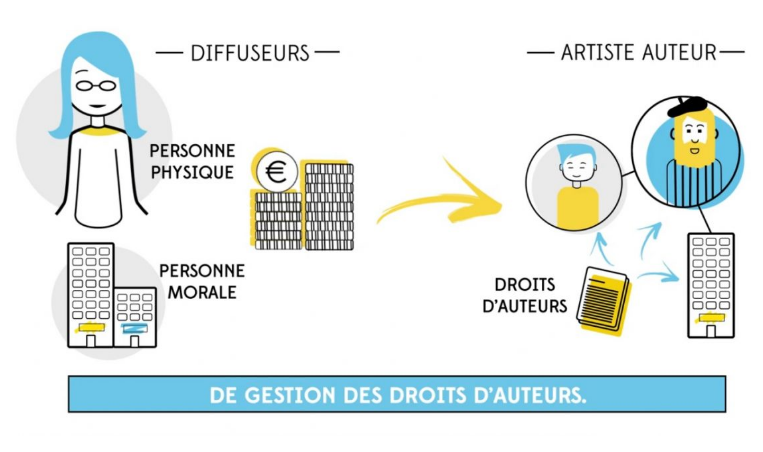
\includegraphics[width=0.8\linewidth]{images/DroitsAuteur.png}
    \caption{Gestion des droits d'auteurs}
\end{figure}

\section{Diagramme des interactions}
\begin{figure}[h!]
    \centering
    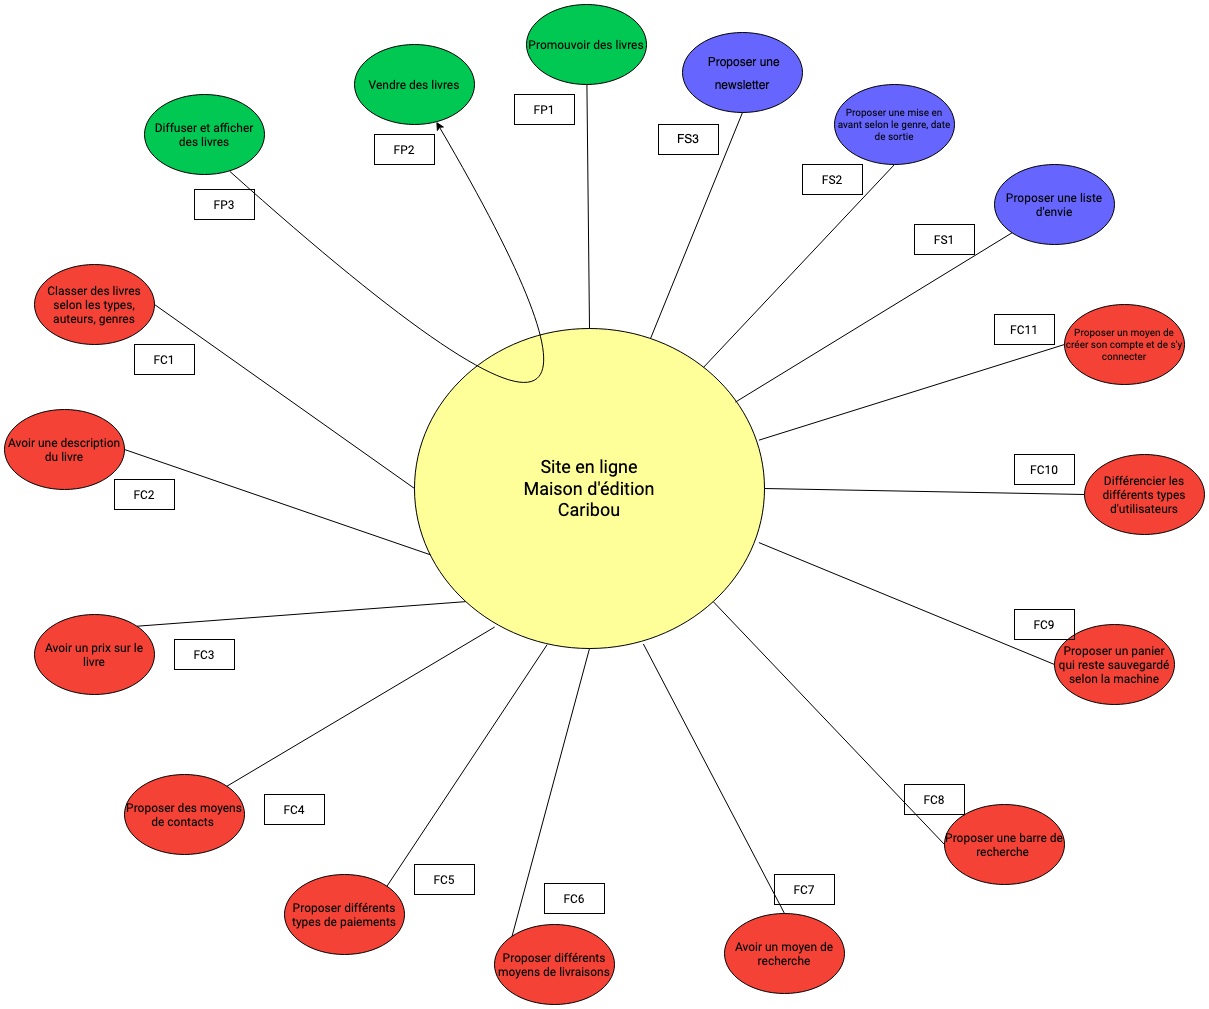
\includegraphics[width=0.8\linewidth]{images/diag_pieuvre.png}
    \caption{Diagramme des interactions\label{fig:Figure2}}
\end{figure}

\section{Analyse fonctionnelle}
\subsection{Fonction principale}
\begin{itemize}
    \item Diffuser et proposer des livres
    \item Vendre des livres physiques et électroniques
\end{itemize}


\subsection{Contraintes}
\begin{itemize}
    \item Classer des livres selon les types, auteurs, genres
    \item Avoir une description du livre (synopsis, taille, genre, etc)
    \item Avoir un prix sur le livre
    \item Proposer différents types de paiements
    \item Proposer des moyens de contacts (email, numéro de téléphone)
    \item Proposer différents moyens de livraisons (à l'adresse, point-relais)
    \item Avoir un moyen de recherche (selon le type, auteur, genre, etc)
    \item Proposer une barre de recherche (nom du livre, auteur)
    \item Proposer un panier (achats groupés) qui reste sauvegardé selon la machine
    \item Différencier les différents types d'utilisateurs (clients, administrateurs)
    \item Proposer un moyen de créer son compte et de s'y connecter
\end{itemize}

\subsection{Fonctions secondaires}
\begin{itemize}
    \item Proposer une newsletter
    \item Proposer une mise en avant selon le genre, date de sortie
\end{itemize}
\end{document}